\chapter{RSVP and MPLS-DiffServ-TE}

In this chapter we will present an overview of a set of technologies that offer a tight control on QoS.
This control comes at the price of complexity, but the ISPs and the manufacturers have decided that QoS is worth it.
This technologies offer control on the path followed by the packets, bandwidth reservation (and therefore guarantees) and fast re-route capabilities.

\section{Multi Protocol Label Switching (MPLS)}

In the IP paradigm, the routers forward the packets based on the destination IP of the packet.
MPLS offers a completely different alterative, in which the forwarding is not done using the destination address.
Instead, labels are used at each hop to decide the outgoing interface.
This approach is called ``virtual circuit packet network'' as it somehow emulates a circuit on a packet network, and it is opposed to the ``datagram'' IP paradigm.
The virtual circuit approach has some advantages and disadvantages compared to the datagram approach.

In the MPLS jargon, a virtual circuit is called a Label Switched Path (LSP).
Each of the packets has a header which is called ``the label''.
In fact, a packet may contain multiple labels and it is said that they are ``stackable''.
The last label can be found on top.

Upon reception of a packet, the outermost label is inspected.
Each router has a lookup table indicating, for every incoming label, the outcoming label and the outcoming interface.
The rooter simply performs the lookup, pops the outermost label and pushes a new label before forwarding the packet.
To populate the lookup table, the LSP is established before starting forwading packets.

In MPLS, the routers are called Label Switch Routers (LSR) and the edge routers Label Edge Routers (LER).
The LSP is established between two LER and then all the packets in the LSP follow exactly the same path.

MPLS is protocol agnostic in the sense that can carry any kind of packets.
Examples are IP packets and Ethernet packets.
This functionality can be used to create both Layer-3 and Layer-2 virtual private networks.
MPLS simply sticks a label on top of any packet (ethernet, IP, etc.)  in the LER which is the entry point of the MPLS domain.
This MPLS packet is forwarded by MPLS by looking only to the label.
The label is removed (popped) at the last or penultimate hop of the MPLS domain.

One of the advantages of MPLS is that the same core can be used to transmit any kind of data.
Another advantage is that it makes it possible to control the path that the packets follow.
The engineering of the paths that the data streams follow within the data networks is called traffic engineering (TE).

\section{Traffic Engineering}

Consider the example scenario in Fig. \ref{fig:traffic-engineering}.
All the links are of 100 Mbps and a propagation delay of 10 ms.
The only exception is link $B-C$ that has a larger delay.
Imagine that you have to carry two streams from router $A$ to router $D$.
One of the streams is a 25 Mbps VoIP stream that requires low delay, jitter and loss.
The second stream is a 80 Mbps stream for remote backup that does not have tight delay and jitter requirements.

\begin{figure}[!h]
\centering
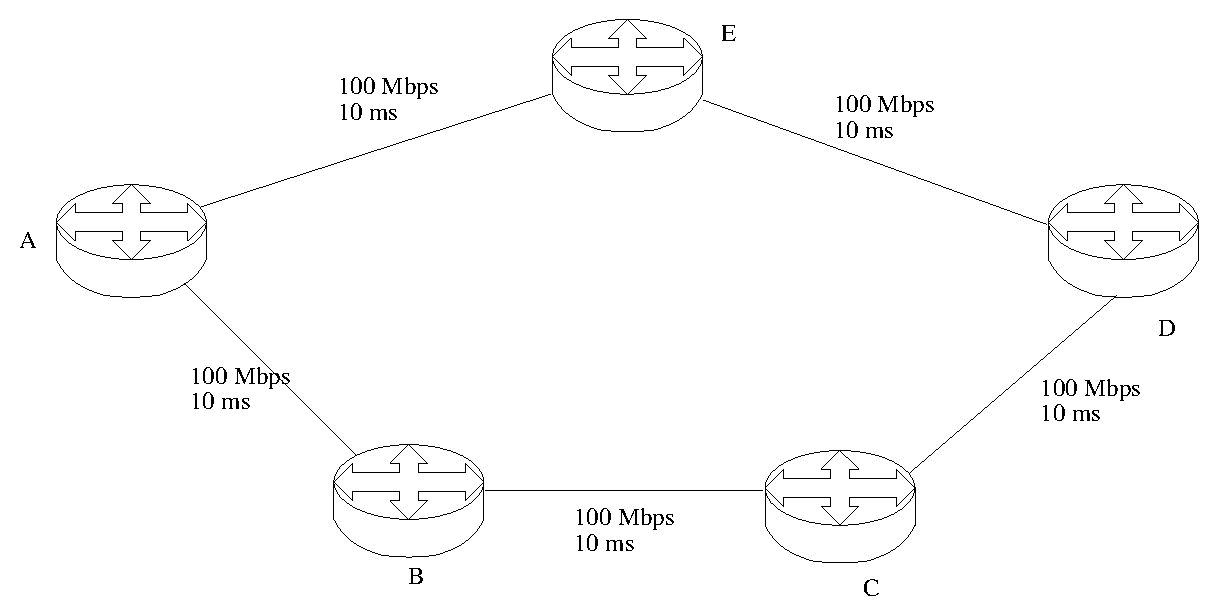
\includegraphics[width=\linewidth]{figures/traffic-engineering.eps}
\caption{Example scenario to explain traffic engineering.}
\label{fig:traffic-engineering}
\end{figure}

The best route between $A$ and $D$ is $A-E-D$.
It has the same bandwidth, less hops, and less total delay than the alternative path $A-B-C-D$.

A datagram-oriented network would choose the best route for all the packet.
Notice that this might not be the best of ideas.
If we direct a total of 105 Mbps (25 of VoIP + 80 of backup data) to 100 Mbps links, queues will build up, and delay, jitter and packet loss will be high.

A better alternative is to direct the 25 Mbps of VoIP traffic to the short path $A-E-D$ and the 80 Mbps of backup traffic to the long link $A-B-C-D$.
Using this solution, we make a better use of our network resources.
All links are utilized, and they are all below 100\% utilization.
This solution provides lower delay, jitter and packet loss for all classes of traffic, as the queues will not build up.

This distribution of data streams in the network is called traffic engineering (TE).
Two reason to engage in TE is to balance the load among different parts of the network to prevent that some links are overloaded while others are empty.
TE is also useful to prevent that delay sensitive streams cross high-latency links (such as satellite links).
Finally, if combined with bandwidth reservation, it can provide guarantees which are important to meet the SLAs that are common in virtual private network services.

\section{Virtual Private Networks using MPLS}
It is common that companies have different sites.
Imagine that a company has a site in the city of Girona and another site in the city of Tarragona.
This company wishes to have a single network shared among the two sites.
The option of deploying a fiber to connect the two sites might be an overkill.
Another option might be to approach an ISP and pay for a ``virtual connection'' between the two sites.

This virtual connection is described in terms of a rate, a burst size and a delay.
The company can push a packet in Girona, and it will ``magically'' appear in Tarragona.
In reality, the ISP will establish a LSP between the two sites.
The ISP takes the packet received in Girona, sticks a label on to the packet, and it switches it through the network until it reaches Tarragona.
Note that it does not matter what the packet is.
Whatever it is, it will be taken from one site and delivered to the other.

From the company's perspective, it is exactly the same as having a pipe that connects the two sites.
In order to guarantee a given bandwidth and delay, the ISP must make a reservation in all the packets that are traversed by the LSP from Girona to Tarragona.
This reservation has to be in terms of bandwidth and buffer space to accommodate the burst size.
The protocol used to make the reservation for the LSP of the VPN is called ``Resource Reservation Protocol for Traffic Engineering'' (RSVP-TE).


\section{Bandwidth reservation and RSVP-TE}
When a new LSP needs to be established, the first step is to decide the path that it will take.
This step is performed with the constrained shortest past first (CSPF) protocol.
CSPF is very similar to the popular open shortest path first (OSPF) protocol.
The only difference is that in CSPF we can apply some constraints to prune the tree.

This constraints can be placed in terms of bandwidth availability or ``colors''.
The ``colors'' simply mark a given property of a link.
As an example, a network administrator might decide to mark the high-latency link in Fig. \ref{fig:traffic-engineering} as ``red''.
Then, when looking for a path for the VoIP link, CSPF can take into account that ``red'' links must be avoided.
In fact, CSPF prunes all the links that do not satisfy the constraints and then uses OSPF in the remaining topology.

The protocol that is used for bandwidth reservation along the path is RSVP-TE.
The LER at the network entry point of the LSP sends a RSVP-TE ``path'' message to the endpoint.
This message is forwarded using CSPF along the path that the LSP will follow. 
Each router in the path, adds his identifier to the path message.
This information will be used to populate the forwarding table.

When the ``path'' messages reaches the LSP tailend, the tailend router creates a ``rsvp'' message that will traverse exactly the same path as the ``path'' message but in the opposite direction.
The ``rsvp'' message is the one that actually creates the reservation.
The only purpose of the ``path'' message is to mark the forward path.
Remember that the paths on a data network are not necessarily symmetrical.
For this reason, it is needed that the ``path'' message if forwarded using the routing protocol from the headend to the tailend.
The ``rsvp'' message is not forwarded using the routing protocol, but with the information gathered by the ``path'' message.

The ``path'' and the ``rsvp'' messages contain the information about the stream, in terms of data rate and bucket size.
The ``rsvp'' makes the actual reservation and it is also used for each router to indicate the label it will use to receive the packets of the LSP.
As an example, if a LSP is established through the routers $A-E-D$ in Fig. \ref{fig:traffic-engineering}, the tailend router $D$ will say in his RSVP message to $E$:
``I am expecting to receive the packets marked with label 123''.
And $E$ will tell to $A$: ``I am expecting to receive the packets marked with label 121''.
And $E$ will include an entry to its lookup table with this information: ``When I receive a packet through the interface connected to $A$ with the label 121, I will swap the label to 123 and I will forward it to the interface connected to router $D$''.
Router $E$ will also reserve the bandwidth and the buffer space required for the stream, and distribute the updated information of its available resources.
Note that these actions take place in the control plane. 
It might be necessary to include a policer in the network entrypoint to ensure that the streams adhere to traffic profile (rate/bucket depth) that they have reserved.


The RSVP-TE protocol has a soft-state, which means that it is maintained as long as it is refreshed by ``path'' and ``rsvp'' messages.
If none of this messages is received for a long time, the router cancels the reservation and frees the resources.

The combination of selecting the path (using CSPF) and reserving router resources makes it possible to offer the guarantees agreed upon in the SLA.
If no path is found that satisfies the criteria, or one of the routers cannot commit the requested resources (because the CSPF path has been computed with outdated information), the LSP cannot be established.

RSVP-TE includes another ingredient which is the priority of a LSP.
A LSP of higher priority can preempt a lower priority LSP.
The low priority LSP then has to look for an alternative path.
In the creation and destruction of LSPs, the ``make before break'' rule is always applied, to make sure that no traffic is blackholed.

It is a common practice to assign higher priorities to larger (or more restrictive) streams, as smaller streams (or streams with lesser restrictions) are easier to accommodate.
It is like filling a car's trunk. 
People normally starts by putting the largest suitcases and then fitting the smaller ones in the empty spaces.

\section{Fast Re-Route}

One of the QoS requirements is availability.
In case of failure, is it important to restore network services as soon as possible.
The kind of traffic with more stringent requirements is VoIP.
A network failure that lasts for more than 50 ms might be noticed by the users of a VoIP conversation.

The protocols exchange ``hello'' messages with their neighbours to detect failures.
If a router stops receiving the periodical hello messages from a neighbour it means that something is going wrong.
Additionally, RSVP has built mechanisms to signal the failure of a path.
When the headend of the LSP is notified of the failure, it can re-compute the path when the routing protocol has re-converged.

The only problem is that all this process, specially routing re-convergence, can take more than a second.
And we would like to have path restoration below 50 ms.
The solution is that, upon failure, a ``patch'' is applied to the path in the form of a ``detour''.
The packets will be forwarded around the failed node or link until a new LSP is created.
The ``patched'' LSP will be destroyed when the brand new LSP is operative, in a ``make before break'' fashion.

\section{MPLS-DiffServ-TE}

So far we have not discussed per-hop-behaviours in the context MPLS-TE.  
If we want to have different classes of traffic and different PHB, is it interesting to take them into account when making reservations.
A clear example is the use of EF for VoIP and the rule of not devoting more than 30\% of the bandwidth to this class.

In the reservation process, we are not interested on how much bandwidth is available in a node.
Instead, we are interested of how much EF bandwidth it is available.
MPLS-DiffServ-TE provides the extensions to make the reservations on a per-class basis.
Obviously, it is also necessary to distribute the information of bandwidth availability for the different classes.

